\lab{Algorithms}{Complexity and Sparse Matrices}{Complexity and Sparse Matrices}

\objective{Introduce the temporal and spatial complexity and explore SciPy's methods for working with sparse matrices.}

\section*{Complexity}
The complexity of an algorithm is how hard it is for a computer to solve. Two major constraints on computing are time and available memory (or ``space''). Hence, when you are evaluating an algorithm, you should ask about its temporal complexity and spatial complexity.

\subsection*{Temporal Complexity}
One of the most important questions in scientific computing is ``How long will a computer take to execute this algorithm?"
For example, suppose an algorithm operating on a 1-D array of length $n$ requires $f(n)$ calculations, where

\begin{equation*}
f(n) = \frac{3n^3}{2} + 75n^2 + 250n + 30.
\end{equation*}

As $n$ increases, the growth of $f(n)$ is dominated by the $n^3$ term.
For this reason we say that $f(n) \in O(n^3)$, or more commonly, that $f(n)$ is $O(n^3)$ (spoken ``Big O of n cubed'' or ``order of n cubed"). So if we double the size of the input $n$, we would expect the algorithm to need about $2^3=8$ times as many steps, which would make it run about 8 times as long.

The function $f(n)$ above is called the \emph{temporal complexity} of the algorithm. In general, $n$ is a positive integer that somehow describes the size of the inputs to your algorithm. For example, perhaps your algorithm accepts $n \times n$ arrays, or perhaps it accepts 1-D arrays of length $n$. The temporal complexity of your algorithm is a function that accepts an input size $n$ and returns the number of steps the algorithm needs to execute on that input. As such, temporal complexity is a precise way to describe how the execution time of your algorithm increases as the size of your input increases.

Often, we do not care about the exact definition of $f(n)$ so much as its behavior when $n$ gets large. This leads to the notion of an \emph{asymptotic upper bound}.
\begin{comment}
\begin{figure}
\centering
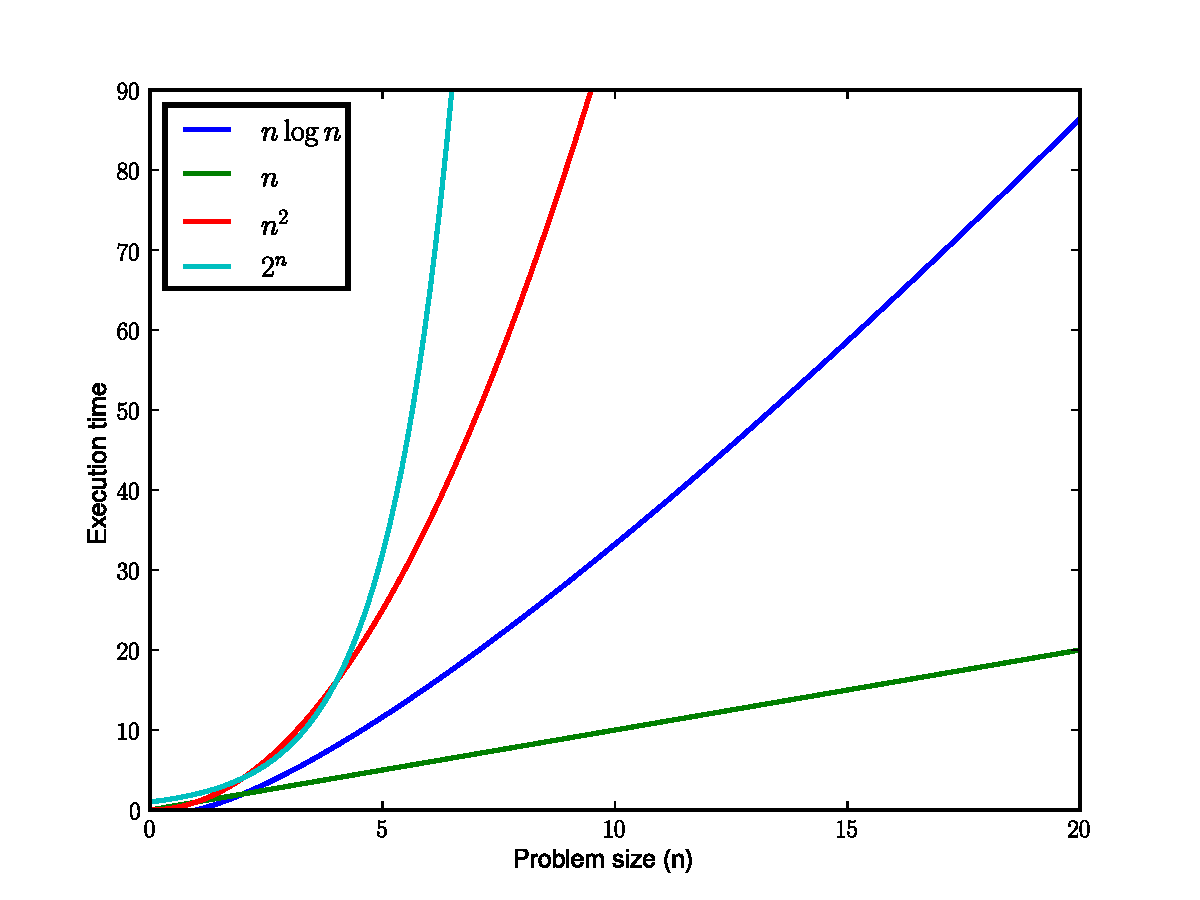
\includegraphics[width=\textwidth]{complexitycurves.pdf}
\caption{Some common asymptotic curves.}
\end{figure}
\end{comment}

\begin{definition}[Assymptotic Upper Bounds]
Let $f(n)$ and $g(n)$ be functions mapping natural numbers to positive real numbers. If there exists a real number $c > 0$ and a natural number $n_0$ such that for all natural numbers $n > n_0$, $f(n) \leq cg(n)$, then $g(n)$ is an \emph{asymptotic upper bound} for $f(n)$. We write $f \in O(g(n))$ or $f = O(g(n))$.
\end{definition}

This vocabulary allows us to mathematically answer the question at the start of this section: ``How long will a computer take to execute this algorithm?". A useful answer is an asymptotic upper bound for the temporal complexity of the function.

For example, adding two $n \times n$ matrices is $O(n^2)$. This is because it takes 1 step to add each pair of elements in two $n \times n$ arrays, and there are $n^2$ such pairs.
By comparison, calculating the inverse of a $n \times n$ matrix using Gaussian
row reduction is $O(n^3)$. (There are more efficient
algorithms for matrix inversion.)

How do we determine the temporal complexity of a piece of code?
Calculating the exact temporal complexity of an algorithm is fairly difficult.
However, there are ways to heuristically evaluate the asymptotic behavior of an algorithm's temporal complexity. For example, consider the following code.

\begin{lstlisting}
s = 0
for i in xrange(n):
    s = s + i
\end{lstlisting}

The code above is $O(n)$ because it takes approximately $n$ steps to complete. For-loops are a good indicator of the complexity.  A double for-loop suggests $O(n^2)$ or worse.  

You can also approximate the temporal complexity of a function by timing how long it takes to run on inputs of various sizes. The ratios of the run times will give you clues about the temporal complexity of the algorithm. For example, if an algorithm is $O(n^3)$, then doubling the size of the input should make the algorithm take $(2n)^3/n^3=8$ times as long.
\begin{comment}
\begin{problem}
Time the runtime of the following code for \li{n = 1000, 2000, 4000, 8000}.

\lstinputlisting[style=fromfile]{test.py}

Now write a function that takes no arguments and does the following: 
\begin{enumerate}
\item Plots the four runtimes (use \li{[1000, 2000, 4000, 8000]} or an equivalent array object as your domain).
The plot should look like Figure \ref{prob1} if using the \li{plt.scatter} command. 
\item Returns the average ratio between successive runtimes (one such ratio would be the runtime for $n = 2000$ divided by the runtime for $n = 1000$).
\end{enumerate}
\begin{figure}
\centering
\includegraphics[width=\textwidth]{prob1.pdf}
\caption{The plot of problem 1}
\label{prob1}
\end{figure}
\end{problem}
\end{comment}

\begin{problem}\label{complexity_ratios}
Fill in the following table. Here, $f(n)$ is the temporal complexity of an algorithm. The quantity $f(2n)/f(n)$ tells you how much longer each algorithm will take to run when you double the size of the input.

\begin{center}
\begin{tabular}{| l |p{15mm}|p{15mm}|p{15mm}|p{15mm}|p{15mm}|}\hline
$f(n)$ & $\log(n)$ & $n\log(n)$ & $n$ & $n^2$ & $2^n$ \\ \hline
$f(2n)/f(n)$&  & & & & \\
\hline
\end{tabular}
\end{center}

\end{problem}

\begin{problem}\label{complexity_timeit}
Determine the temporal complexity of each of the following functions. Do this as follows:
\begin{enumerate}
\item Time how long the function takes to run on an input of size $n$ for $n=1000, 2000, 4000$, and $8000$.
\item Compute the average of the ratios between successive runtimes from part (1).
\item Use Problem \ref{complexity_ratios} to determine the temporal complexity.
\end{enumerate}
\end{problem}

\begin{problem}
Create a plot depicting the complexities you found in Problem \ref{complexity_timeit} by following these steps. 
\begin{enumerate}
\item For each function, plot a line using $n=1000, 2000, 4000$, and $8000$ for $x$-values and your runtimes for $y$-values. When you call the function \li{plt.plot()}, specify a value for the keyword parameter \li{label} so you can reference each line later. For example, the call \li{plt.plot( x, y, label="Function 1")} attaches the label "Function 1" to this line.
\item After plotting all your lines, call \li{plt.legend()} to draw a legend on your graph. Use the keyword argument \li{loc} to specify the location of the legend. Some possible values are \li{'upper left'} and \li{'right'}. See the documentation for more options.
\end{enumerate}
Your graph should look something like this.

[TODO: put a figure here]
\end{problem}



\subsection*{Spatial Complexity}
Analogous to temporal complexity, the spatial complexity of an algorithm is a function that describes how the algorithm's memory use increases as input sizes to the algorithm increase. Spatial and temporal complexity are not completely independent of each other, as the amount of memory required by an algorithm can affect its speed in several ways. The most important way is that when the memory usage exceeds the amount of available RAM, the machine must use the hard disk or some other slower storage method. Therefore, you should try to be aware of how much RAM your algorithm requires. In the next section, we will learn special storage methods that reduce the spatial complexity of handling certain arrays.

\section*{Sparse Matrices}
A \emph{sparse} matrix is a matrix that has relatively few nonzero elements. A matrix with few zero entries is \emph{dense}. The SciPy module \li{sparse} has matrix storage methods that are optimized for sparse matrices. When we are not using these special methods, we say we are storing the \emph{full} matrix. We can also use \li{sparse} methods on dense matrices, but doing so will take longer than using the usual methods for handling full matrices. So, sparse versus dense refers to a property of abstract matrices, and sparse versus full refers to how any matrix is stored in memory, regardless of its abstract properties. You minimize spatial complexity when you store a sparse matrix with the \li{sparse} module and a dense matrix as a full (or ``regular'') matrix.

This difference in spatial complexity comes because a full array occupies a block of memory for each entry,, so a $n \times n$ array requires $n^2$ blocks of memory. By contrast, SciPy's \li{sparse} methods store only the nonzero entries and their locations in the array. As long as most entries are 0 (i.e., the matrix is sparse), this decreases spatial complexity. As listed in Table \ref{smr}, SciPy has 7 different sparse matrix types, corresponding to 7 ways of storing sparse matrices.



\begin{table}[ht]
\centering
\begin{tabular}{|r|l|}
\hline
Sparse Matrix Type & Description \\
\hline
\li{bsr_matrix} & Compressed Block Sparse Row\\
\li{coo_matrix} & Coordinate\\
\li{csc_matrix} & Compressed Sparse Column\\
\li{csr_matrix} & Compress Sparse Row\\
\li{dia_matrix} & Sparse Diagonal\\
\li{dok_matrix} & Dictionary of Keys\\
\li{lil_matrix} & Linked List\\
\hline
\end{tabular}
\caption{Sparse matrix representations in SciPy}
\label{smr}
\end{table}

Let us compare a \li{sparse} matrix computation with a full matrix computation. Note that we can convert any full matrix to a \li{sparse} matrix of any of the types listed in Table \ref{smr}.

\begin{lstlisting}
# Create a dense matrix (stored as a full matrix)
>>> A_full = np.random.rand(600, 600)

# Store A_full as a ``sparse'' matrix (even though it is dense)
>>> A_sparse = sparse.csc_matrix(A_full)

# Create a sparse matrix (stored as a full matrix)
>>> B_full = np.diag( np.random.rand(600) )

# Store B_full as a sparse matrix
>>> B_sparse = sparse.csc_matrix(B_full)

>>> def square(A):
...     return np.power(A, 2)

>>> %timeit square(A_full)
100 loops, best of 3: 9.53 ms per loop

>>> %timeit square(A_sparse)
1 loops, best of 3: 941 ms per loop

>>> %timeit square(B_full)
100 loops, best of 3: 5.36 ms per loop

>>> %timeit square(B_sparse)
1000 loops, best of 3: 259 us per loop
\end{lstlisting}

As you can see from this example, we get the best performance when we store a sparse matrix with the \li{sparse} module and a dense matrix as a full (or ``regular'') matrix.

\begin{comment}
\begin{problem}
Create a $500\times 500$ matrix and vector of length 500, both full of random values. Use the \li{A.dot(b)} command to multiply your matrix and your vector, and time how long it takes to do so. Then convert your matrix to sparse format and again time how long it takes to multiply it by your vector using \li{A.dot(b)}.
\end{problem}
\end{comment}

\subsection*{Creating Sparse Matrices}
One way to create a sparse matrix is to create a full matrix and then convert it to a sparse matrix, as we did in the previous example. However, it is more memory-efficient if you never create the full matrix. Here are two ways to create sparse matrices directly.

The first way is to use the method \li{sparse.spdiags(data, diags, m, n)}. If \li{data} is a 1-D array and \li{diags} is a scalar, then this method creates an $m \times n$ matrix with \li{data} on the specified diagonal. The parameter \li{diags=0} indicates the main diagonal, with lower diagonals indexed by negative numbers and upper diagonals by positive numbers. If \li{data} is a 2-D array and \li{diags} is a list, then this method creates an $m \times n$ matrix with the rows of \li{data} on the diagonals specified by \li{diags}. See the documentation for more information.
\begin{lstlisting}
# Create a sparse 3x3 matrix with (2, 3, 4) on the diagonal
>>> A = sparse.spdiags([2, 3, 4], 0, 3, 3)
>>> A
<3x3 sparse matrix of type '<type 'numpy.int64'>'
	with 3 stored elements (1 diagonals) in DIAgonal format>
# Convert A to a full matrix
>>> A.todense()
matrix([[2, 0, 0],
        [0, 3, 0],
        [0, 0, 4]])
	
# Create a sparse 4x4 matrix with the rows of diag_entries on the diagonals
>>> diag_entries = np.array([[3,6,9,0],[1,4,7,10],[0,2,5,8]])
>>> B = sparse.spdiags(diag_entries, [-1, 0, 1], 4, 4)
<4x4 sparse matrix of type '<type 'numpy.int64'>'
	with 10 stored elements (3 diagonals) in DIAgonal format>
>>> B.todense()
matrix([[ 1,  2,  0,  0],
        [ 3,  4,  5,  0],
        [ 0,  6,  7,  8],
        [ 0,  0,  9, 10]])
\end{lstlisting}

The final matrix \li{B} in the example above is a special kind of matrix called a \emph{banded} matrix. A banded matrix is a sparse matrix whose only non-zero entries are on the main diagonal and some diagonals on either side. In fact, $B$ is an example of a \emph{tri-diagonal} matrix, because its nonzero entries are confined to the three central diagonals. Banded matrices arise naturally in many applications, including numerical methods for solving differential equations. 

\begin{problem}
Write a function that takes an integer argument \li{n} and returns a sparse $n\times n$
tri-diagonal array in \li{csr_matrix} format with $2$'s along the diagonal and $-1$'s along
the two sub-diagonals above and below the diagonal.
This matrix is the derivative operator in numerical analysis of differential equations.
\emph{Hint}: Read about the \li{format} keyword parameter of the \li{sparse.spdiags()} method.
\label{prob:sparse_tridiag}
\end{problem}

A second way to create a sparse matrix is to pre-allocate an array of zeros and then specify the nonzero entries one at a time. The most efficient sparse matrix type for pre-allocation is \li{lil}. Once you are done constructing the sparse matrix, you should convert it to a form that is more efficient for computations (like \li{csr} or \li{csc}).


\begin{lstlisting}
# Initialize Z
>>> Z = sparse.lil_matrix((400, 300))

# Specify the nonzero entries of Z
>>> Z[1,34] = 23
>>> Z[23,32] = 56
>>> Z[2,:] = 13.2
>>> Z
<400x300 sparse matrix of type '<type 'numpy.float64'>'
	with 302 stored elements in LInked List format>

\end{lstlisting}

When the matrix \li{Z} is initialized, all its entries are assumed to be zero. 
Note that at the end of \li{Z}'s construction, only 302 elements are being stored for a matrix with 120000 entries. 

%insert problem here that lets them play around with large sparse matrices in diff forms


\begin{comment}
\subsection*{Banded Matrices}
\begin{problem}
Write a function that takes an integer argument \li{n} and returns a full $n\times n$
tri-diagonal array with $2$'s along the diagonal and $-1$'s along
the two sub-diagonals above and below the diagonal.
\emph{Helpful Hint}: Use the \li{np.diagflat()} command.
\label{full_tridiag}
\end{problem}
\end{comment}



\section*{Using Sparse Matrices}
As we have discussed, storing a sparse matrix with the \li{sparse} module decreases spatial complexity. Here is an example.

\begin{lstlisting}
>>>B = np.random.rand(3, 10000)
>>> A = sparse.spdiags(B, range(-1, 2), 10000, 10000)

# Only do this if you have several gigabytes of memory
>>> A_dense = A.todense() 

>>> A.data.nbytes # About .24MB of memory.
240000

>>> A_dense.nbytes # About 762.9MB of memory.
800000000

\end{lstlisting}
Storing \li{A} as a dense matrix takes more than 3,000 times as much memory. 

You may have noticed that the only way to view a matrix as a 2-D array is to convert it to a full matrix. If your matrix is too large to do this (as was \li{A} in the previous example),
you can still visualize it using the \li{plt.spy()} command from matplotlib. This function plots
locations of the non-zero entries in a matrix.
Taking \li{A_dense} to be the matrix of the previous example, the output of \li{plt.spy(A_dense)} is shown in Figure \ref{fig:mpl_spy}.

\begin{figure}[ht]
\centering
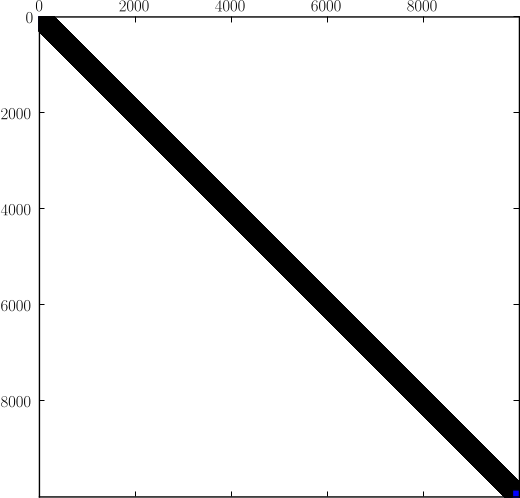
\includegraphics[width=10cm]{spy.png}
\caption{The output of the \li{spy()} command}
\label{fig:mpl_spy}
\end{figure}




In addition to spatial complexity, the \li{sparse} module can reduce temporal complexity. Consider the linear system $A x = b$, where $A$ is a $100000\times 100000$ tri-diagonal matrix.
Storing a full matrix of that size requires 10 billion double-precision floating-point numbers.  Since it takes 8 bytes to store a double, we need roughly 80GB to store the full matrix.  Lack of storage space makes this system impossible to solve for most desktop computers, but even more problematic is the temporal complexity.
Methods for directly solving a linear system are usually $O(n^3)$. As a result, even if the computer could store an 80GB matrix in RAM, it would still take several weeks to solve the system. 
%However, since we don't typically have computers with that much available RAM, most of the
%matrix would have to be stored on the hard drive, so the computation would probably take between $6$ months to a year.

The point is, even as computers increase in processing speed and memory, we can still easily construct problems that they will struggle to solve in a reasonable amount of time. However, if we store the tri-diagonal matrix as a \li{sparse} matrix, we can solve the linear system, even with a modest computer.  

Let's first compute the spatial complexity of the above system when $A$ is stored as a sparse matrix.  There are three diagonals that have roughly $100000$ non-zero entries.  That's $300000$
double-precision floating point numbers, which is about 2.4 MB, or less storage than your favorite song.  Thus, the sparse matrix will easily fit into the computer's RAM.  Furthermore, the temporal complexity for solving a tri-diagonal matrix is $O(n)$. Let's see how long it takes to solve the system when $A$ and $b$ are filled with random data.

\begin{lstlisting}
>>> from scipy.sparse import linalg as sl
>>> D = np.random.rand(3, 100000)
>>> b = np.random.rand(1, 100000)
>>> A = sparse.spdiags(D,[-1,0,1],100000,100000, format='csr')
>>> def solSys():
...     return sl.spsolve(A, b)

>>> %timeit solSys()
1 loops, best of 3: 80.8 ms per loop

\end{lstlisting}

This computer solved the system in only 80.8 milliseconds.

\begin{problem}
Write a function that accepts an integer argument \li{n} as well as a keyword argument \li{sparse} whose value is either \li{True} or \li{False} (default to \li{False}). Then do the following:
\begin{enumerate}
\item Inside of the function, use your previous solutions to generate an $n \times n$ tri-diagonal array $A$ -- either sparse or full depending on the value of the \li{sparse} argument.
\item Generate an $n \times 1$ random array $b$
\item Solve the system $Ax = b$, using either \li{scipy.sparse.linalg.spsolve} or \li{scipy.linalg.solve}
(again depending on the value of \li{sparse}) and return the solution.
\item Time the function for \li{n = 2000} using both the sparse and the full option.
\end{enumerate}
\end{problem}

\begin{problem}
Write a function that accepts an integer argument \li{n} and returns $\lambda n^2$, where
$\lambda$ is the smallest eigenvalue of the same $n \times n$ sparse tri-diagonal array as described above.

To calculate $\lambda$, use \li{scipy.sparse.linalg.eigs}. You will need to set the \li{which = 'SM'}
optional argument. If \li{A} is your tri-diagonal sparse matrix, you will need to use
\li{A.asfptype()} as the argument for the \li{eigs} function (so that the matrix has the right data type).
Check the documentation of the \li{eigs} function to see what it returns, so that you will know how to
get the smallest eigenvalue.

What value does $\lambda n^2$ approach as $n \rightarrow \infty$?

\li{Helpful Hint}: It's the square of an important number.
This is related to operator theory: the second derivative operator has this eigenvalue in certain cases.
\end{problem}





 
